%%%%%%%%%%%%%%%%%%%%%%%%%%%%%%%%%%%%%%%%%%%%%%%%%%%%%%%%%%%
%\documentclass[xcolor=x11names,compress]{beamer}
\documentclass[xcolor=x11names,aspectratio=169, compress]{beamer}
%% General document
\usepackage{graphicx, subfig}
%% Beamer Layout
\useoutertheme[subsection=false,shadow]{miniframes}
\useinnertheme{default}
\usefonttheme{serif}
\usepackage{palatino}

%%%%%%% Mes Packages %%%%%%%%%%%%%%%%
%\usepackage[french]{babel}
\usepackage[T1]{fontenc}
\usepackage{color}
\usepackage{xcolor}
\usepackage{dsfont} % Pour indicatrice
\usepackage{url}
\usepackage{multirow}
\usepackage[normalem]{ulem}   % For strike out text

% Natbib for clean bibliography
\usepackage[comma,authoryear]{natbib}

%remove the icon
\setbeamertemplate{bibliography item}{}

%remove line breaks
\setbeamertemplate{bibliography entry title}{}
\setbeamertemplate{bibliography entry location}{}
\setbeamertemplate{bibliography entry note}{}

%% ------ MEs couleurs --------
\definecolor{vert}{rgb}{0.1,0.7,0.2}
\definecolor{brique}{rgb}{0.7,0.16,0.16}
\definecolor{gris}{rgb}{0.7, 0.75, 0.71}
\definecolor{grisplus}{rgb}{0.5, 0.5, 0.5}
\definecolor{twitterblue}{rgb}{0, 0.42, 0.58}
\definecolor{airforceblue}{rgb}{0.36, 0.54, 0.66}
\definecolor{siap}{RGB}{3,133, 200}


%%%%%%%%%%%%%%%%% BEAMER PACKAGE %%%%%%%

\setbeamercolor{itemize item}{fg=siap}
%\setbeamercolor{itemize subitem}{fg=blue}
%\setbeamercolor{itemize subsubitem}{fg=cyan}

\setbeamercolor{enumerate item}{fg=siap}

\setbeamerfont{title like}{shape=\scshape}
\setbeamerfont{frametitle}{shape=\scshape}

\setbeamercolor*{lower separation line head}{bg=DeepSkyBlue4}
\setbeamercolor*{normal text}{fg=black,bg=white}
\setbeamercolor*{alerted text}{fg=siap}
\setbeamercolor*{example text}{fg=black}
\setbeamercolor*{structure}{fg=black}
\setbeamercolor*{palette tertiary}{fg=black,bg=black!10}
\setbeamercolor*{palette quaternary}{fg=black,bg=black!10}

% Set the header color to SIAP's color
\setbeamercolor*{frametitle}{fg=siap}

%remove navigation symbols
\setbeamertemplate{navigation symbols}{}

\renewcommand{\(}{\begin{columns}}
\renewcommand{\)}{\end{columns}}
\newcommand{\<}[1]{\begin{column}{#1}}
\renewcommand{\>}{\end{column}}

%% Add footer with logo
\setbeamertemplate{footline}{%
  \begin{beamercolorbox}[wd=\paperwidth,ht=2.5ex,dp=1.125ex,%
    leftskip=.3cm,rightskip=.3cm plus1fil]{author in head/foot}
    
\includegraphics[height=5ex]{SIAP_logo_Big.png}\hfill
    \insertshortauthor\hfill\insertshorttitle\hfill  \textcolor{siap}{\textit{\insertframenumber}}
  \end{beamercolorbox}%
}


% Path for the graphs
\graphicspath{{Graphics/}
{c:/Chris/Visualisation/Presentations/Graphics/Logos/}
{../../Visualisation/Presentations/Graphics/}
{c:/Gitmain/MLCourse/UNML/Module0/M0_files/figure-html/}
{c:/Chris/UN-ESCAP/MyCourses2022/MLOS2022/Slides/Graphics/}
{c:/Chris/UN-ESCAP/MyCourses2023/BigDataKostat/Slides/Graphics/}
{c:/Chris/UN-ESCAP/MyCourses2024/WebScrapping/Graphics/}
 }

\title{\textcolor{siap}{Big Data and Data Science for  Gender Statistics in Asia and the Pacific\\ \vspace{0.5cm} }}

\subtitle{\textcolor{brique}{\Large{Geospatial Data and Methods}}}
\author{Christophe Bontemps}
\institute{ 
\includegraphics[height=10ex]{SIAP_logo_Big.png}}
\date{}

\begin{document}

% Slide 1: Title Slide
\begin{frame}
    \titlepage
\end{frame}


\section{Introduction}

\begin{frame}
{ \Large \color{siap}{Foreword }}
\vspace{0.5cm}

\vspace{0.5cm}
\begin{center}
\emph{“Most of the new data capture technologies and solutions to be presented at the 2023 Forum are enabled by geospatial information systems”} \\
\end{center}

\vspace{1cm}
\color{grisplus}{
\emph{\textbf{Stefan Schweinfest},\\
 Director, UN Statistics Division (UNSD) - Hangzhou, 2023}}

\end{frame}

\begin{frame}
    \frametitle{Introduction}
    \begin{columns}[T]
        \begin{column}{0.7\textwidth}
            \begin{itemize}[<+->]
                \item Geospatial data is a very important source of information for SDGs
                \item Many indicators have an individual component and so \textbf{are} \emph{spatial}
                \item[$\hookrightarrow$] Many indicators are reported through maps
                \item Help measure \textbf{where} progress is, or \textbf{where} to help
                \item Some information can \textbf{only} be collected from sky (environment, infrastructure, ...)
                \item Growing literature on using Satellite images for SDGs and gender statistics
            \end{itemize}
        \end{column}
        \begin{column}{0.3\textwidth}
            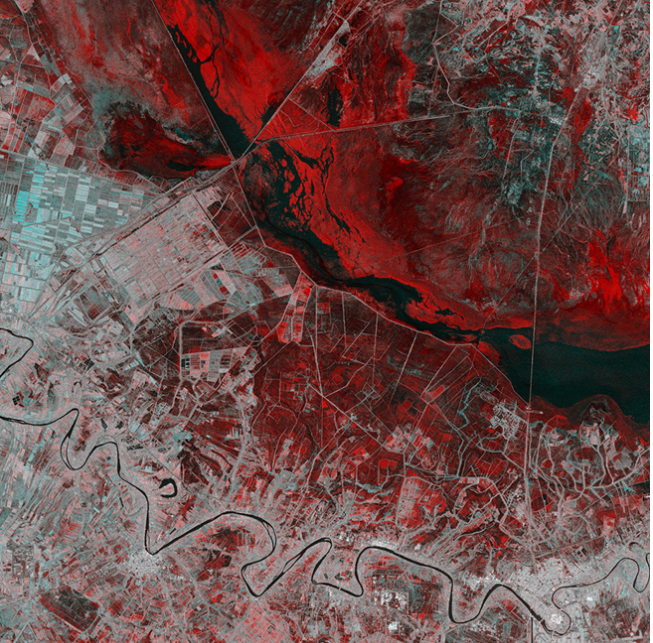
\includegraphics[width=\textwidth]{SpatialImageRed.PNG}
             \textcolor{gris}{\footnotesize{Source: Unitar}}
        \end{column}
    \end{columns}
\end{frame}

\section{Motivation}

\begin{frame}
    \frametitle{Why Geospatial data? }
    Geospatial data can:
    \begin{columns}[T]
        \begin{column}{0.7\textwidth}
            \begin{itemize}[<+->]
            \item Enables spatially targeted policies and interventions $\rightarrow$ \textbf{Where?}
            \item Improves resource allocation by \textbf{identifying areas} of need and vulnerability. $\rightarrow$ \textbf{Who?}
            \item Enhances monitoring and evaluation of gender issues and progress at regional and global levels.$\rightarrow$ \textbf{Why?}
            \item Facilitates evidence-based decision-making by \textbf{integrating} spatial data with other socio-economic indicators. $\rightarrow$ \textbf{How?}
            \end{itemize}
        \end{column}
        \begin{column}{0.3\textwidth}
            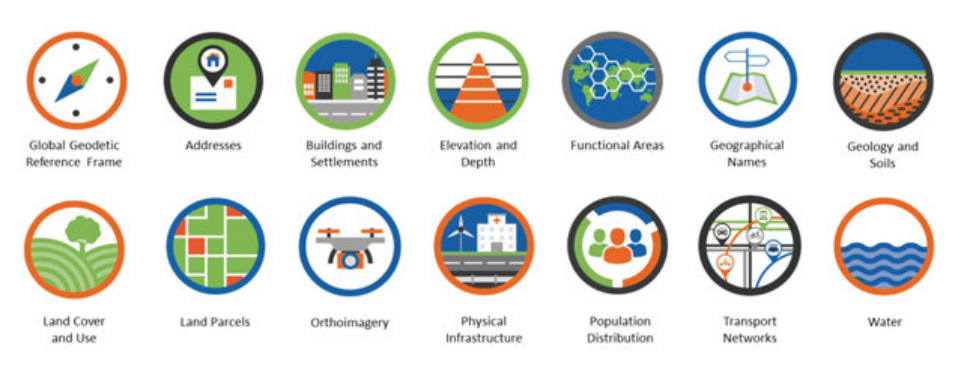
\includegraphics[width=\textwidth]{GeospatialInformation.PNG}
        \end{column}
    \end{columns}
\end{frame}

\begin{frame}
    \frametitle{Types of Geospatial Data}
    \begin{columns}[T]
        \begin{column}{0.7\textwidth}
            \begin{itemize}[<+->]
                \item Satellite imagery: Provides high-resolution images of Earth's surface.
                \item Remote sensing data: Captures information about land cover, vegetation, and environmental changes.
                \item Geographical Information System (GIS) data: Includes boundaries, roads, rivers, and other spatial features.
                \item Global Positioning System (GPS) data: Enables precise location tracking and mapping.
            \end{itemize}
        \end{column}
        \begin{column}{0.3\textwidth}
            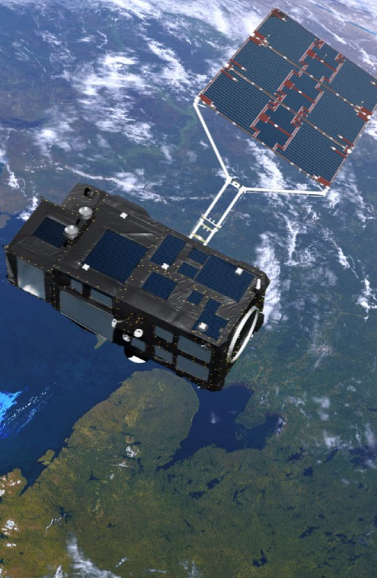
\includegraphics[width=\textwidth]{Satellite.PNG}
        \end{column}
    \end{columns}
\end{frame}

\section{Methods}

\begin{frame}
    \frametitle{Steps for Geospatial Analysis}
    \begin{enumerate}[<+->]
        \item Data acquisition: Obtain relevant geospatial datasets from various sources.
        \item Data preprocessing: Clean, transform, normalize
        \item Integration: Format the geospatial data for a GIS or Statistical software
        \item Spatial analysis: Apply statistical and spatial techniques to explore patterns and relationships.
        \item Evaluation:  Critical assessment of results , accuracy
        \item Visualization: Create maps, charts, and interactive visualizations for data interpretation and communication.
        \item Interpretation and decision-making: Derive insights from the analysis to inform policy decisions and actions.
    \end{enumerate}
\end{frame}

\begin{frame}
    \frametitle{Statistical Methods for Geospatial Analysis}
Some (advanced) methods are used
    \begin{columns}[T]
        \begin{column}{0.6\textwidth}
            \begin{itemize}[<+->]
            \item Spatial classification:
            \item[$\hookrightarrow$] Detect areas, patterns, objects
            \item Spatial clustering:
            \item[$\hookrightarrow$] Separate, isolate component
            \item Spatial regression:
            \item[$\hookrightarrow$] Analyze spatial relationships
            \item Data augmentation
            \item[$\hookrightarrow$] Align spatial data with surveys..
            %\item[$\hookrightarrow$] All of that can be embedded in ML
            %\item Dimension reduction: PCA

            \end{itemize}
        \end{column}
        \begin{column}{0.4\textwidth}
            \begin{itemize}
             \item[]
        \only<1-2>{ 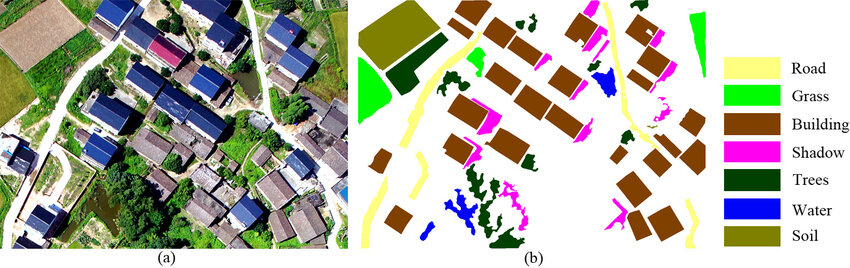
\includegraphics[width=\textwidth]{BuildingClassification.png}  \\
         \textcolor{gris}{\scriptsize{Source: \href{        https://www.researchgate.net/publication/335854050_Novel_Multi-Scale_Filter_Profile-Based_Framework_for_VHR_Remote_Sensing_Image_Classification
}{Lv \emph{et al.} }}}}
        \only<3-4>{ 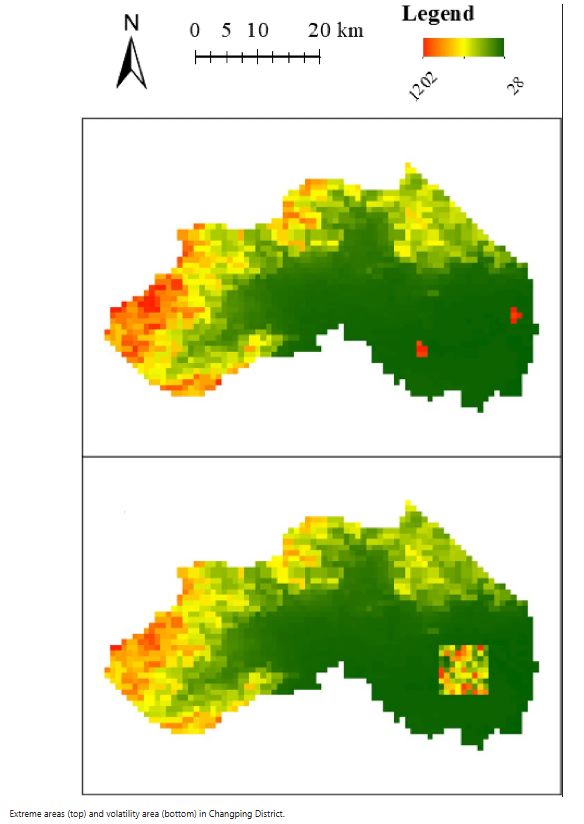
\includegraphics[width=0.9\textwidth]{SpatialClustering.PNG}  \\
                     \textcolor{gris}{\scriptsize{Source: \href{        https://www.nature.com/articles/s41598-024-53066-4}{Wang \emph{et al.} }}}}
        \only<5-6>{ 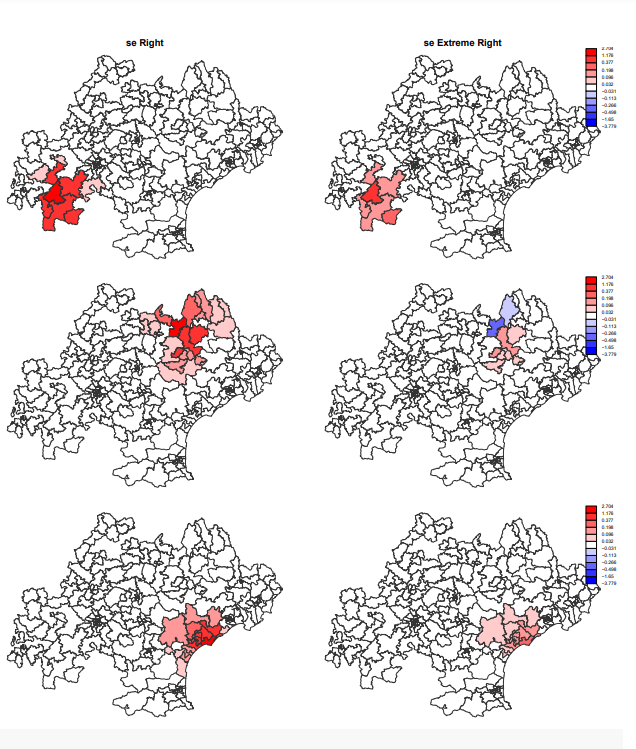
\includegraphics[width=0.9\textwidth]{SpatialRegression.PNG}  \\
                     \textcolor{gris}{\scriptsize{Source: \href{        https://link.springer.com/article/10.1007/s43071-023-00035-0}{Laurent \emph{et al.} }}}}
        \only<7-8>{ 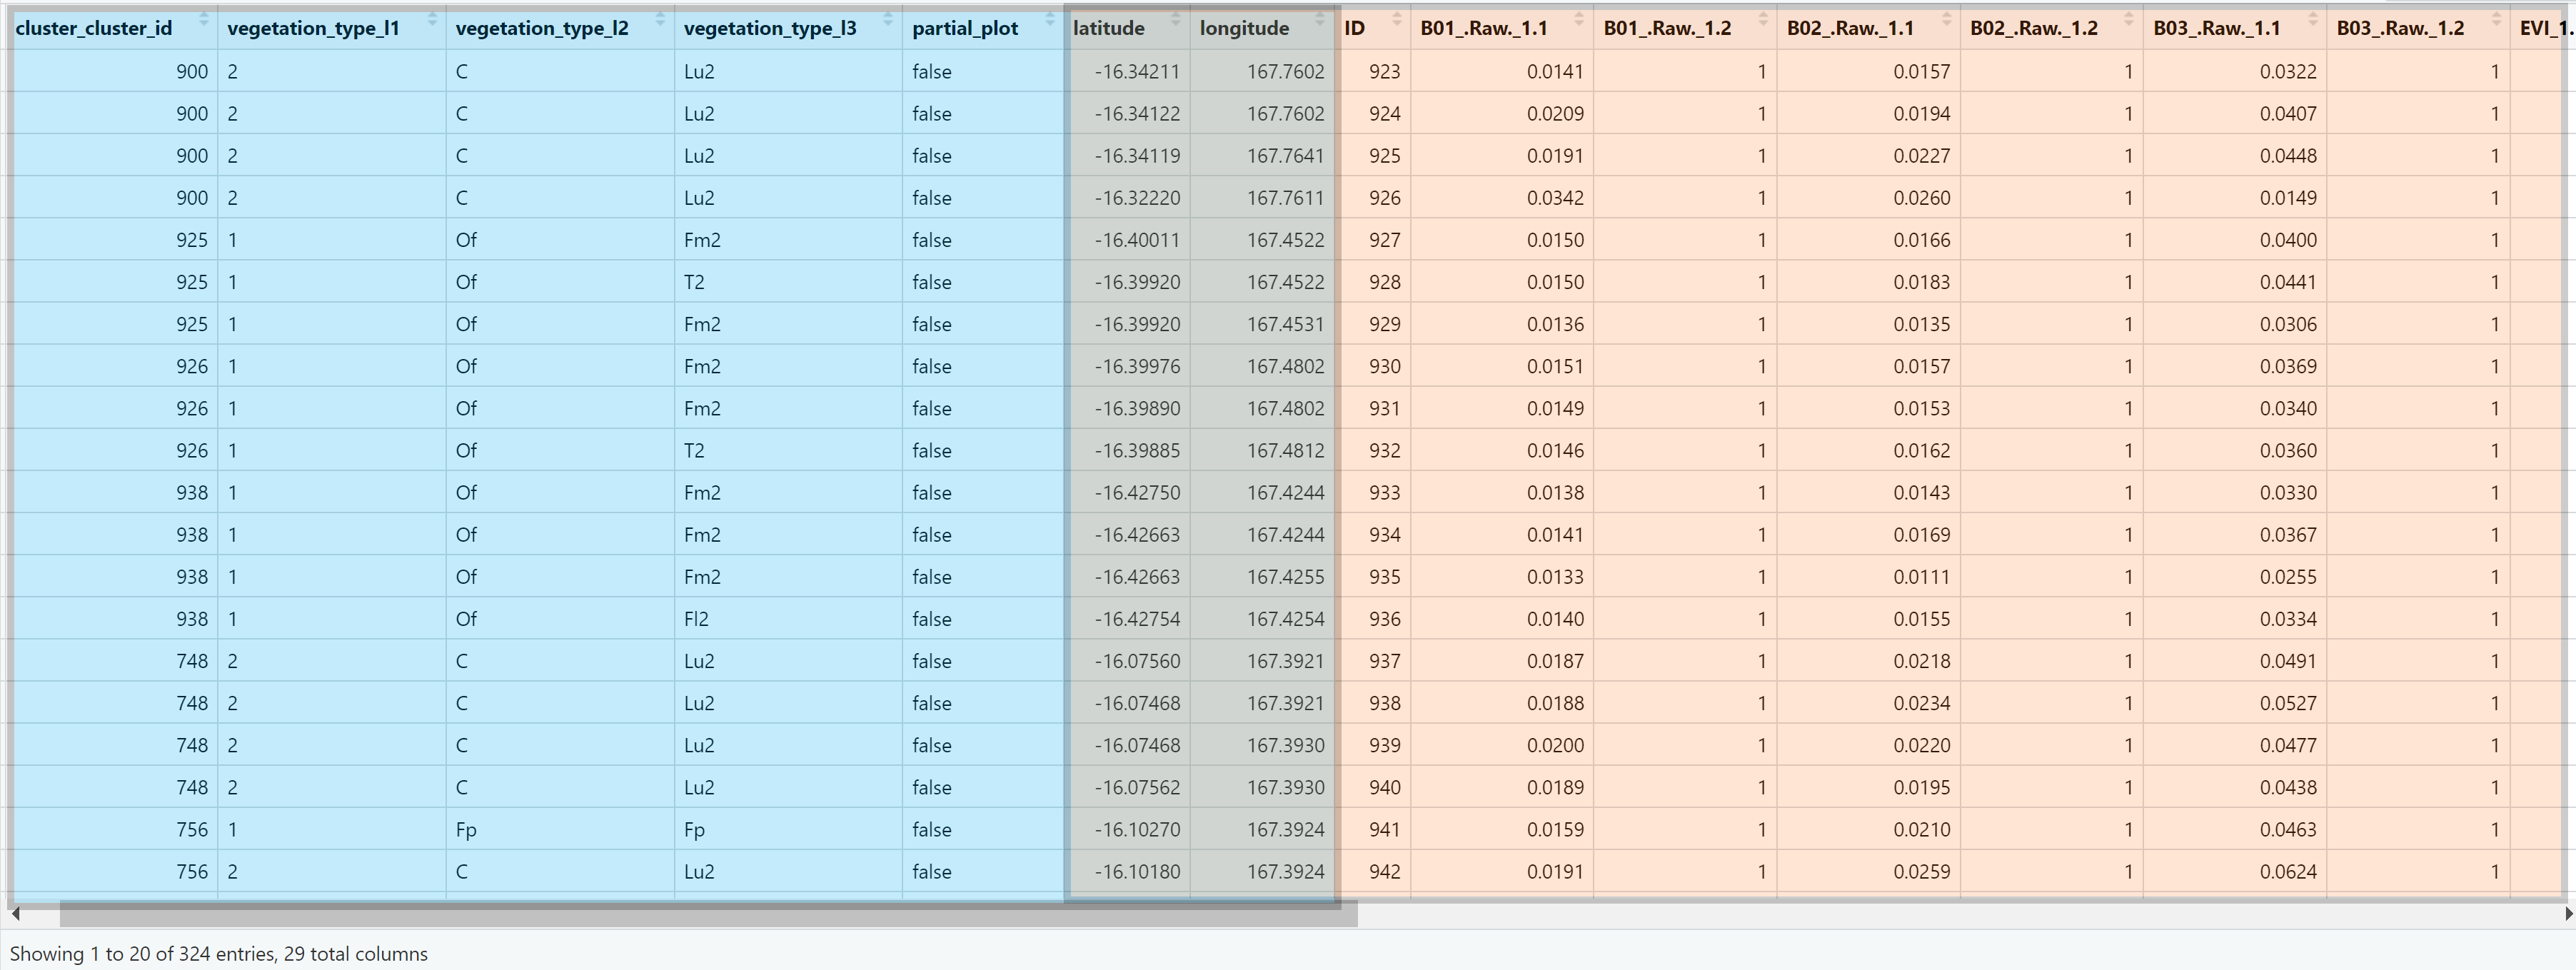
\includegraphics[width=1.0\textwidth]{TableJoined.png}}
            \end{itemize}

        \end{column}
    \end{columns}
\end{frame}

\section{Satellite Imagery }

\begin{frame}
    \frametitle{Working with Geospatial data  }
There are \textbf{two ways} to encode spatial information:\\
\begin{center} \emph{\textbf{Raster} vs \textbf{Vector}} formats  \end{center}
\pause
    \begin{columns}[T]
        \begin{column}{0.6\textwidth}
            \begin{itemize}[<+->]
            \item[$\hookrightarrow$] \textbf{Encode} geography differently
             \item Raster: $\rightarrow $  Matrix or pixel representation
             \item[$\hookrightarrow$] Each cell is stored by its position
             \item[$\hookrightarrow$] Cell size determines the resolution
             \item Vector:  $\rightarrow $  Traditional geographical objects
             \item[$\hookrightarrow$] Efficient encoding
             \item[$\hookrightarrow$] Original resolution and form
            \end{itemize}
        \end{column}
        \begin{column}{0.4\textwidth}
        \begin{itemize}
             \item[]
             \only<2>{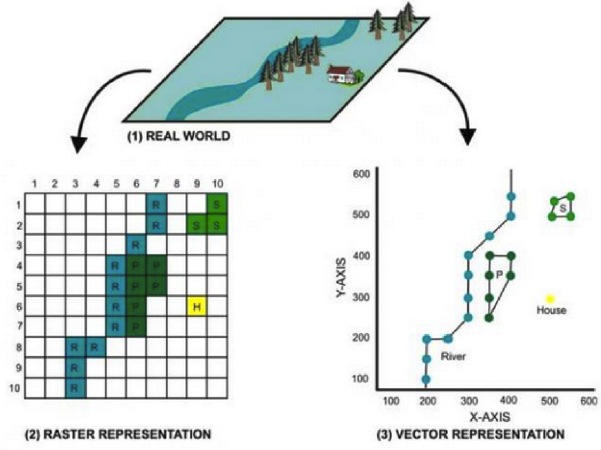
\includegraphics[width=0.9\textwidth]{VectorVsRaster.png} \\ }
             \only<3-5>{ 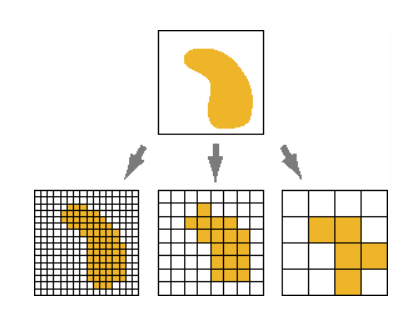
\includegraphics[width=0.9\textwidth]{Raster.png} \\  }
             \only<6-8>{  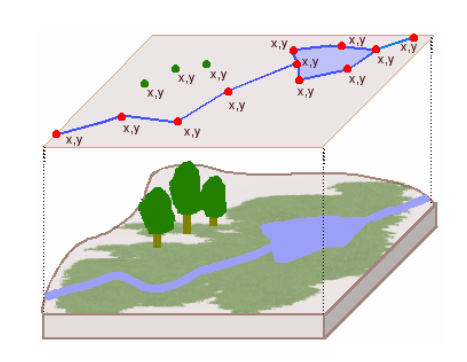
\includegraphics[width=0.9\textwidth]{Vector.png}\\  }
              \only<6-8>{   \textcolor{gris}{\footnotesize{Source: \href{https://desktop.arcgis.com/en/arcmap/10.3/manage-data/raster-and-images/what-is-raster-data.htm}{Arcgis}}} }
        \end{itemize}
        \end{column}
    \end{columns}
\end{frame}

\begin{frame}
    \frametitle{What can  Satellite see? }
    \begin{columns}[T]
        \begin{column}{0.7\textwidth}
            \begin{itemize}[<+->]
             \item Images are made of pixels
             \item[$\hookrightarrow$] Raster!
             \item Satellites have different resolutions (0.5m to  50-250m)
             \item Images are taken at a certain angle:\\ 0 = \emph{Nadir}, else = \emph{off-Nadir} angle
             \item Satellite images are multi- spectral: Radar, infrared, NTL, etc...
             \item Satellite have orbits and time resolution
            \end{itemize}
        \end{column}
        \begin{column}{0.3\textwidth}
         \begin{itemize}
             \item[]
             \only<2>{ 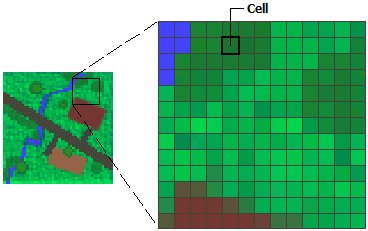
\includegraphics[width=0.9\textwidth]{ImagePixel.png} \\ }
             \only<3>{ 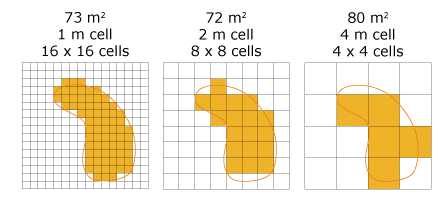
\includegraphics[width=\textwidth]{RasterResolution.png} \\  }
             \only<4>{  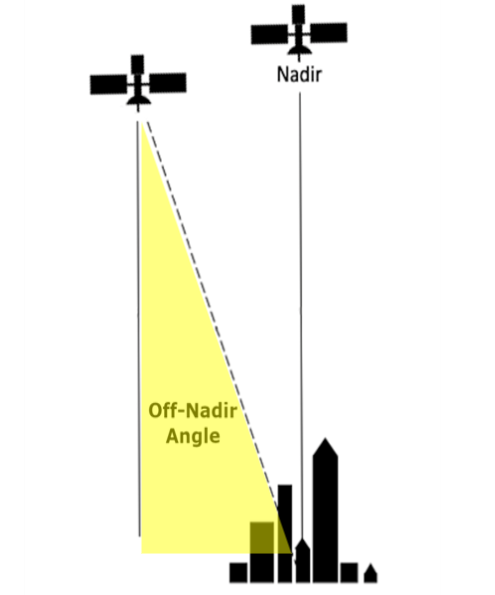
\includegraphics[width=\textwidth]{SpatialAngle.PNG}\\  }
             \only<5>{  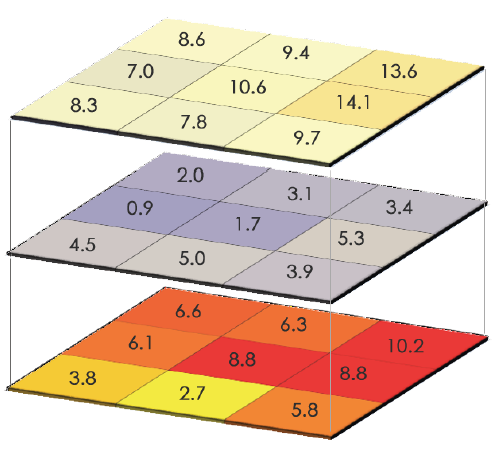
\includegraphics[width=\textwidth]{RasterLayers.png} \\
                        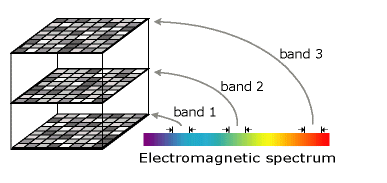
\includegraphics[width=\textwidth]{RasterBands.png} \\ }
             \only<6>{  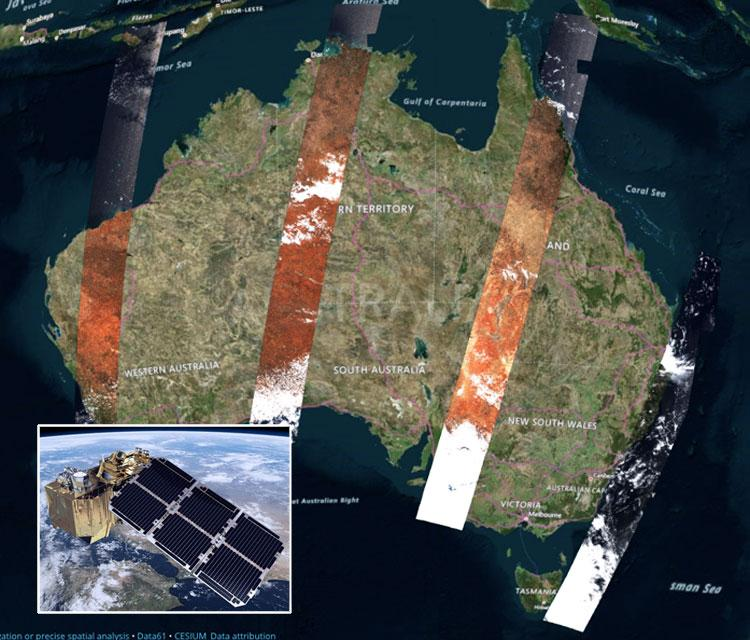
\includegraphics[width=\textwidth]{SatellitePaths.jpg} \\ }

             \only<1-5>{   \textcolor{gris}{\footnotesize{Source: \href{https://pro.arcgis.com/en/pro-app/latest/help/data/imagery/an-overview-of-trajectory-data.htm}{Arcgis}}} }
        \end{itemize}

        \end{column}
    \end{columns}
\end{frame}

\begin{frame}
    \frametitle{Combining Vector and Raster }
How to match different geospatial information
%\pause
    \begin{columns}[T]
        \begin{column}{0.6\textwidth}
            \begin{itemize}[<+->]
            \item Ensure same reference for encoding location (projection)
             \item[$\hookrightarrow$] Align positions
             \item Define the output format
             \item[$\hookrightarrow$] \emph{"Flat"} tables for analysis
             %\item[$\hookrightarrow$] Vectors for GIS tools and maps
             \item Simple example: How to align:
             \item[$\hookrightarrow$] Raster (pixels) with some information
             \item[$\hookrightarrow$] GPS points or zones from DHS (simple vectors)
             \item[]
            \end{itemize}
        \end{column}
        \begin{column}{0.4\textwidth}
        \begin{itemize}
             \item[]
             \only<1-2>{ 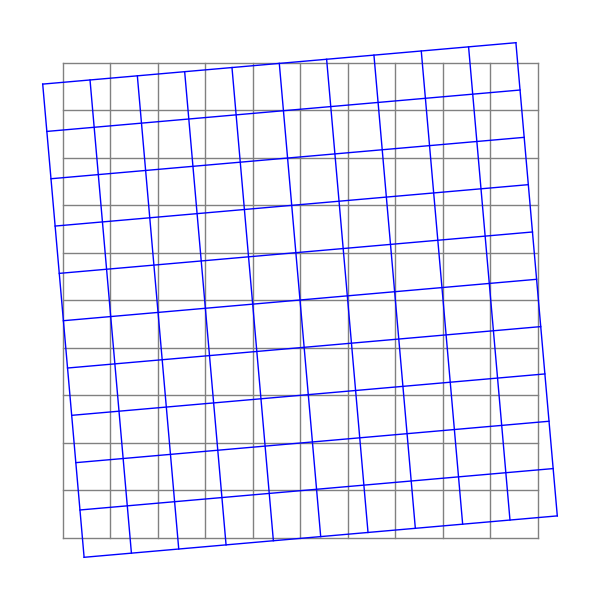
\includegraphics[width=0.9\textwidth]{MisalignedGrids.png} \\ }
             \only<3-4>{ 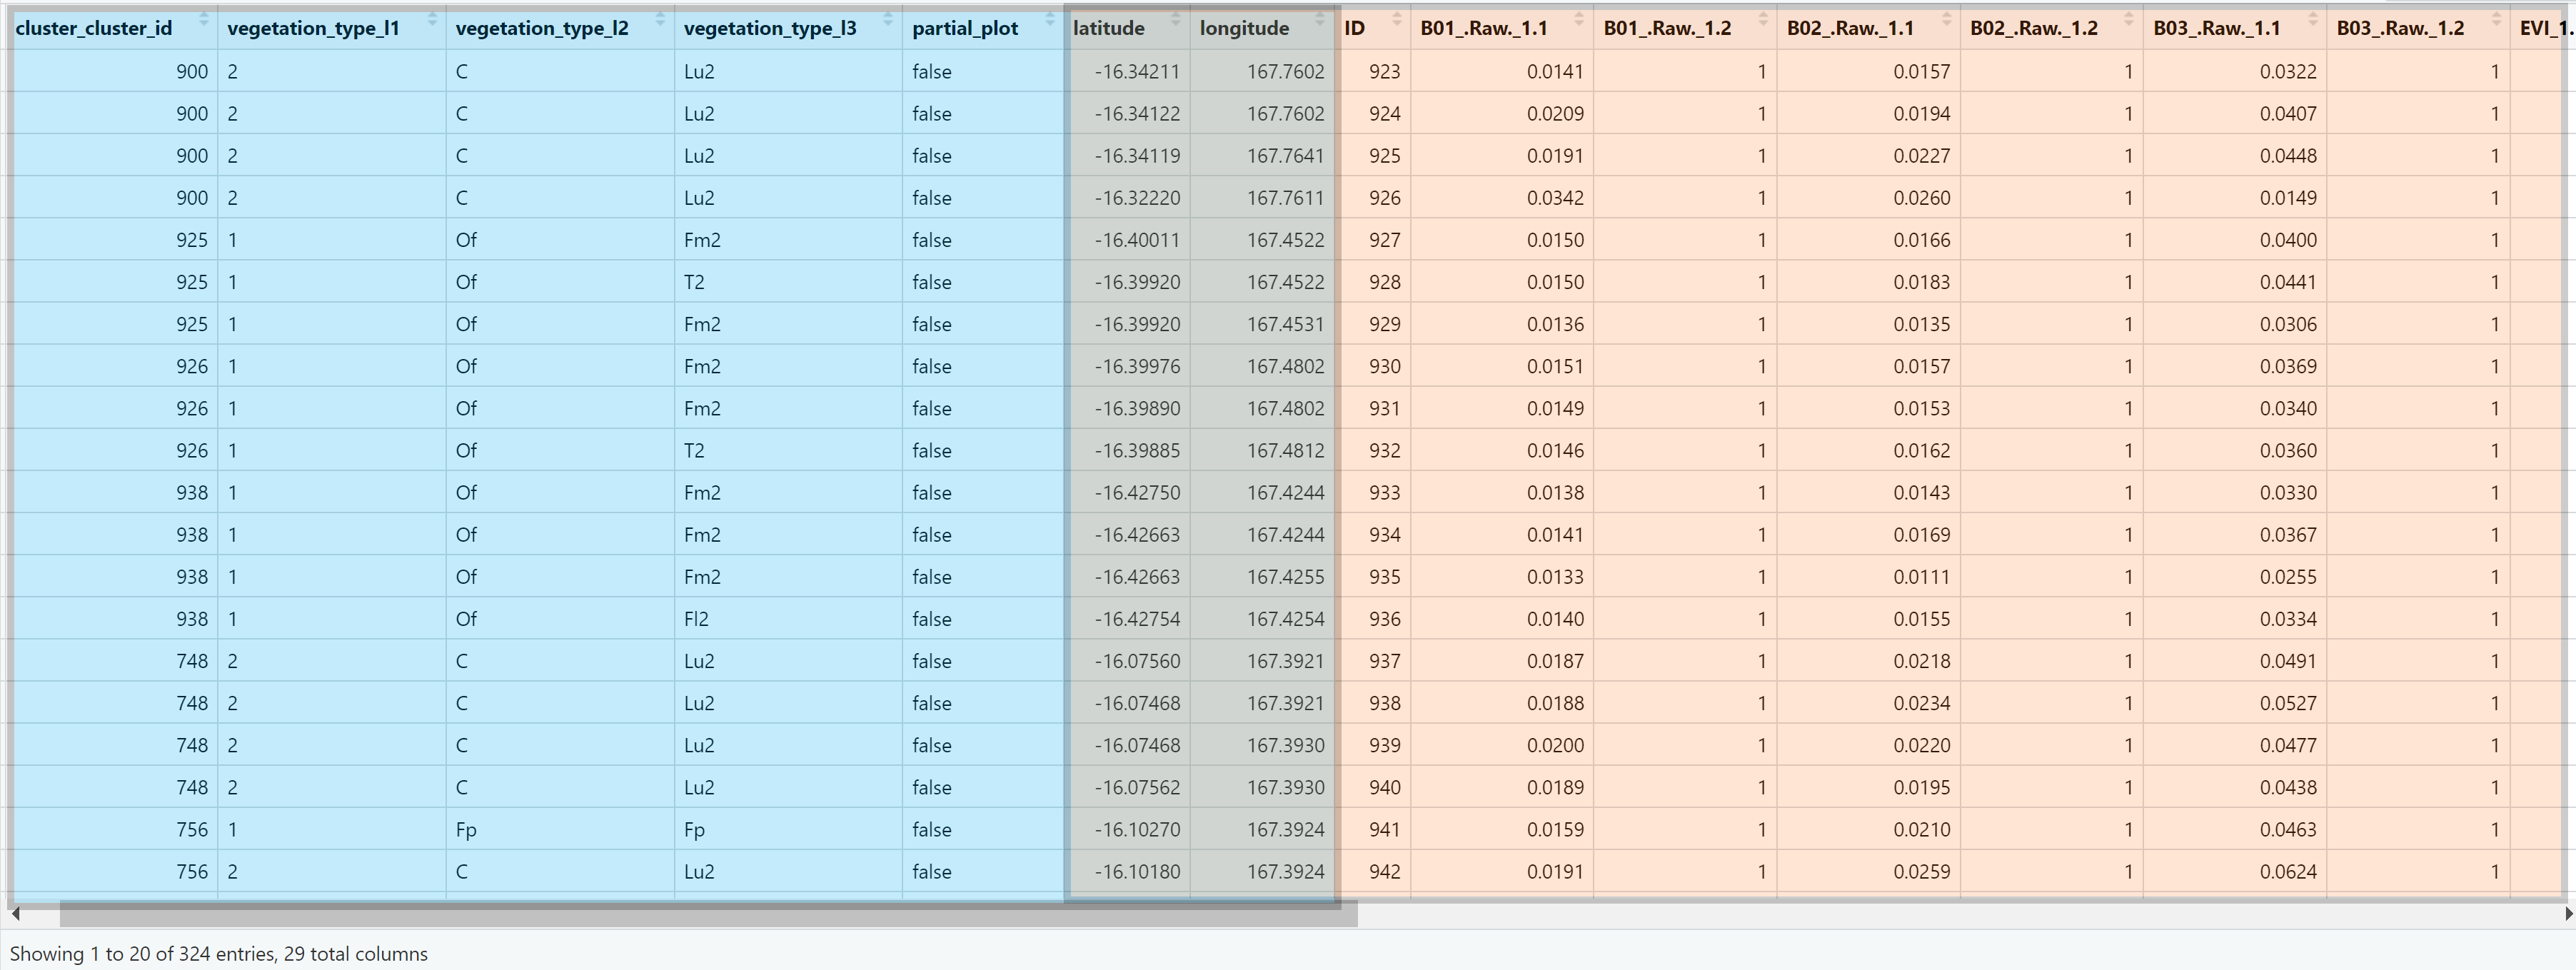
\includegraphics[width=\textwidth]{TableJoined.png} \\  }
             \only<8>{ 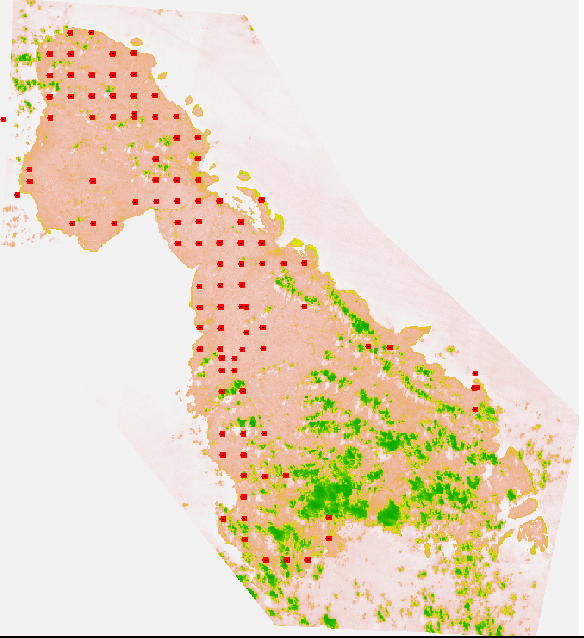
\includegraphics[width=\textwidth]{VMerge.png} \\  }
             \only<6>{ 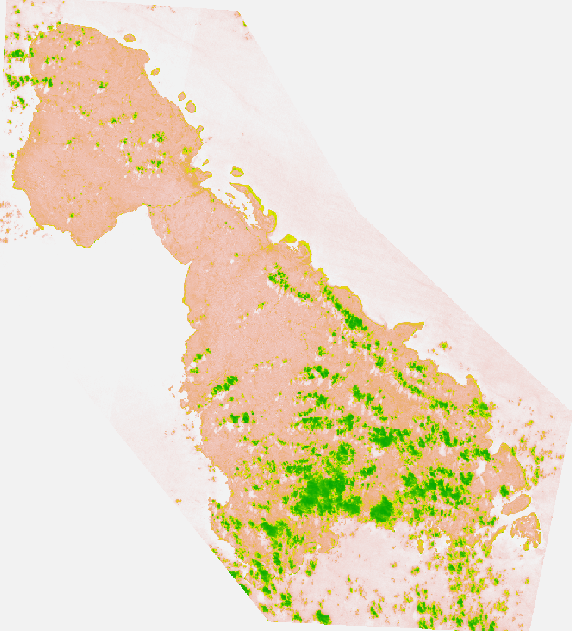
\includegraphics[width=\textwidth]{VRaster.png} \\  }
             \only<7>{ 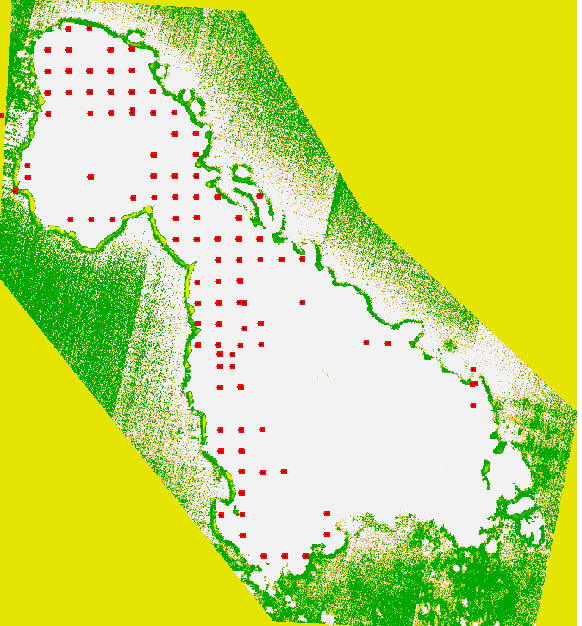
\includegraphics[width=\textwidth]{VPoints.png} \\  }
             %\only<6>{ 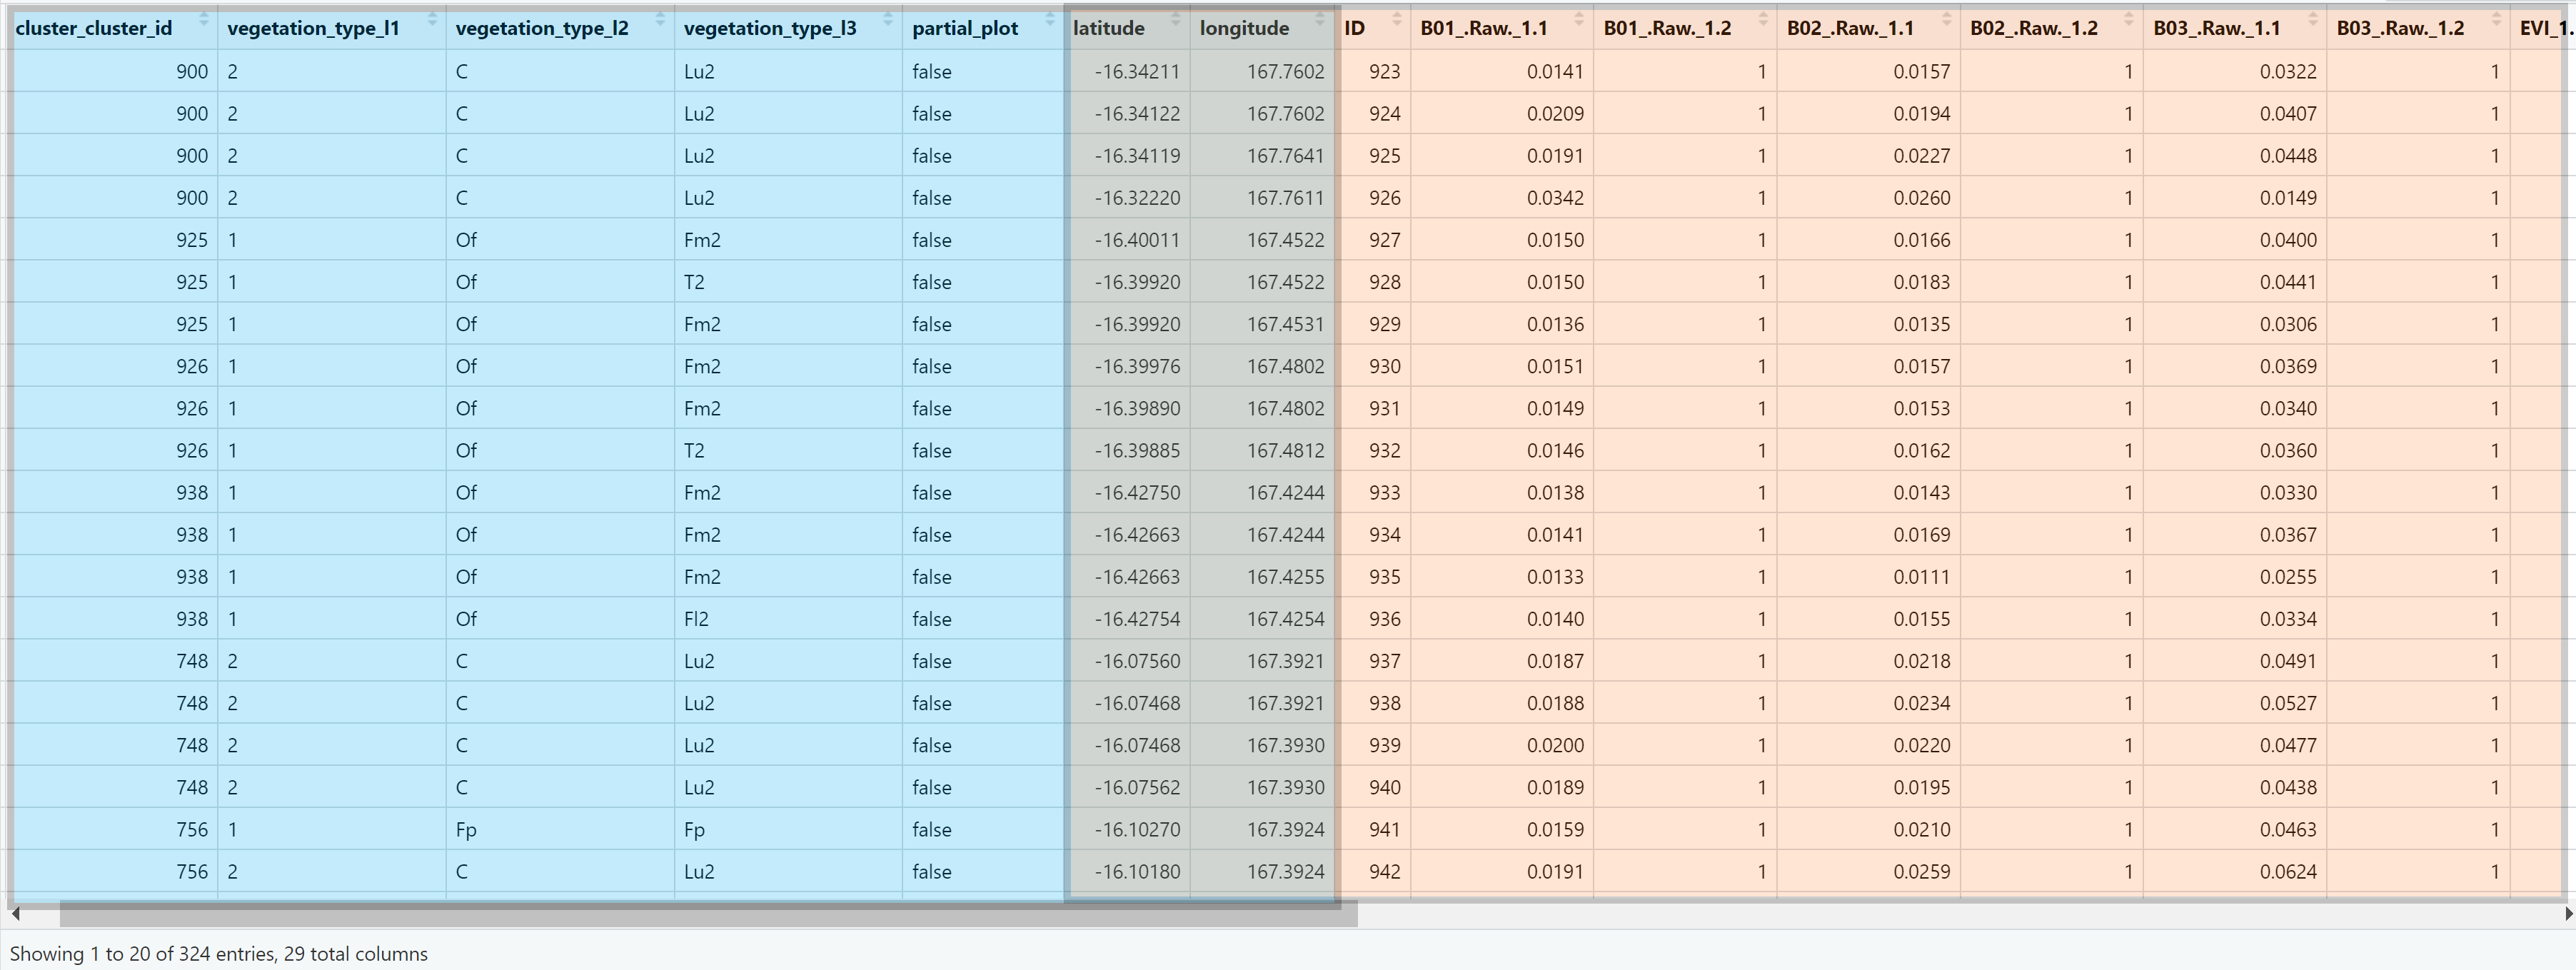
\includegraphics[width=\textwidth]{TableJoined.png} \\ }
             %\only<5-7>{   \textcolor{gris}{\footnotesize{Source: \href{https://desktop.arcgis.com/en/arcmap/10.3/manage-data/raster-and-images/what-is-raster-data.htm}{Arcgis}}} }
        \end{itemize}
        \end{column}
    \end{columns}
\end{frame}

%\section{Limitations}

\begin{frame}
    \frametitle{Limitations}
    \begin{columns}[T]
        \begin{column}{0.7\textwidth}
            \begin{itemize}[<+->]
                \item Data quality: Geospatial can be inaccurate (gaps, outdated, clouds).
                \item Data compatibility: Challenging  integration of different formats, projections and resolutions
                \item Technical skills: Requires specialized knowledge of GIS tools and statistical techniques.
                \item Computational resources: Analysis may require significant computational power and storage capacity.
                \item Privacy and ethics: Handling geospatial data raises privacy concerns and ethical considerations.
            \end{itemize}
        \end{column}
        \begin{column}{0.3\textwidth}
            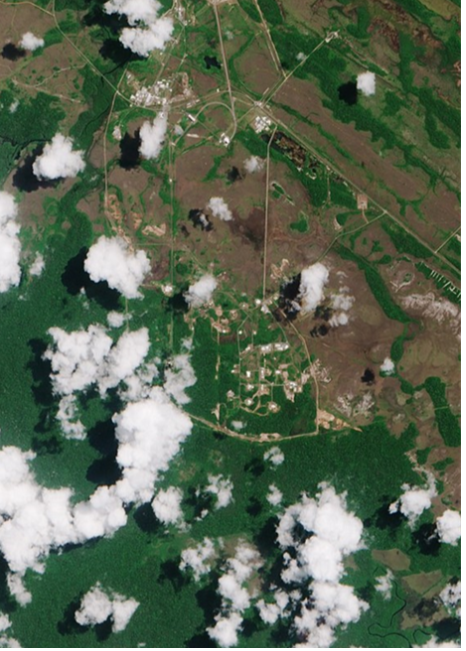
\includegraphics[width=\textwidth]{Clouds.PNG}
        \end{column}
    \end{columns}
\end{frame}

\section{Tools \& sources}

\begin{frame}
    \frametitle{What is a GIS?}
A GIS is a tool used to capture, store, analyze, and display geographically referenced data.
\pause
    \begin{columns}[T]
        \begin{column}{0.5\textwidth}
            \begin{itemize}[<+->]
                \item A GIS can handle different formats of  geospatial information
                \item A GIS can transform different CRS, formats and maps
                \item It can structure information in layers
                \item QGIS is an open-source GIS software
                \item R can do that too (but is more limited)
            \end{itemize}
        \end{column}
        \begin{column}{0.5\textwidth}
        \begin{itemize}
             \item[]
             \only<2>{
             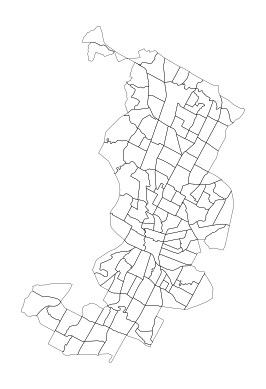
\includegraphics[width=0.25\textwidth]{AreaGISInformation1.png} 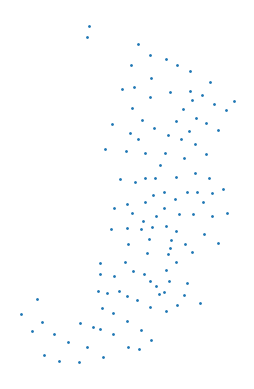
\includegraphics[width=0.25\textwidth]{AreaGISInformation2.png} \\
             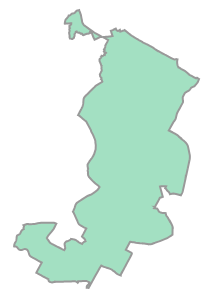
\includegraphics[width=0.25\textwidth]{AreaGISInformation3.png}
             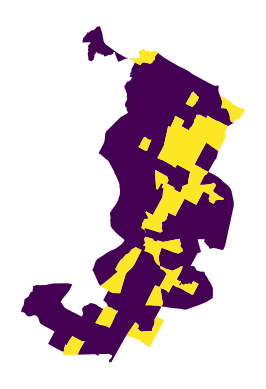
\includegraphics[width=0.25\textwidth]{AreaGISInformation4.png} \\
              \textcolor{gris}{\footnotesize{Source:
             \href{https://pythongis.org/part2/chapter-06/nb/02-geometric-operations.html}{GIS Python}}} \\  }
             \only<3>{ 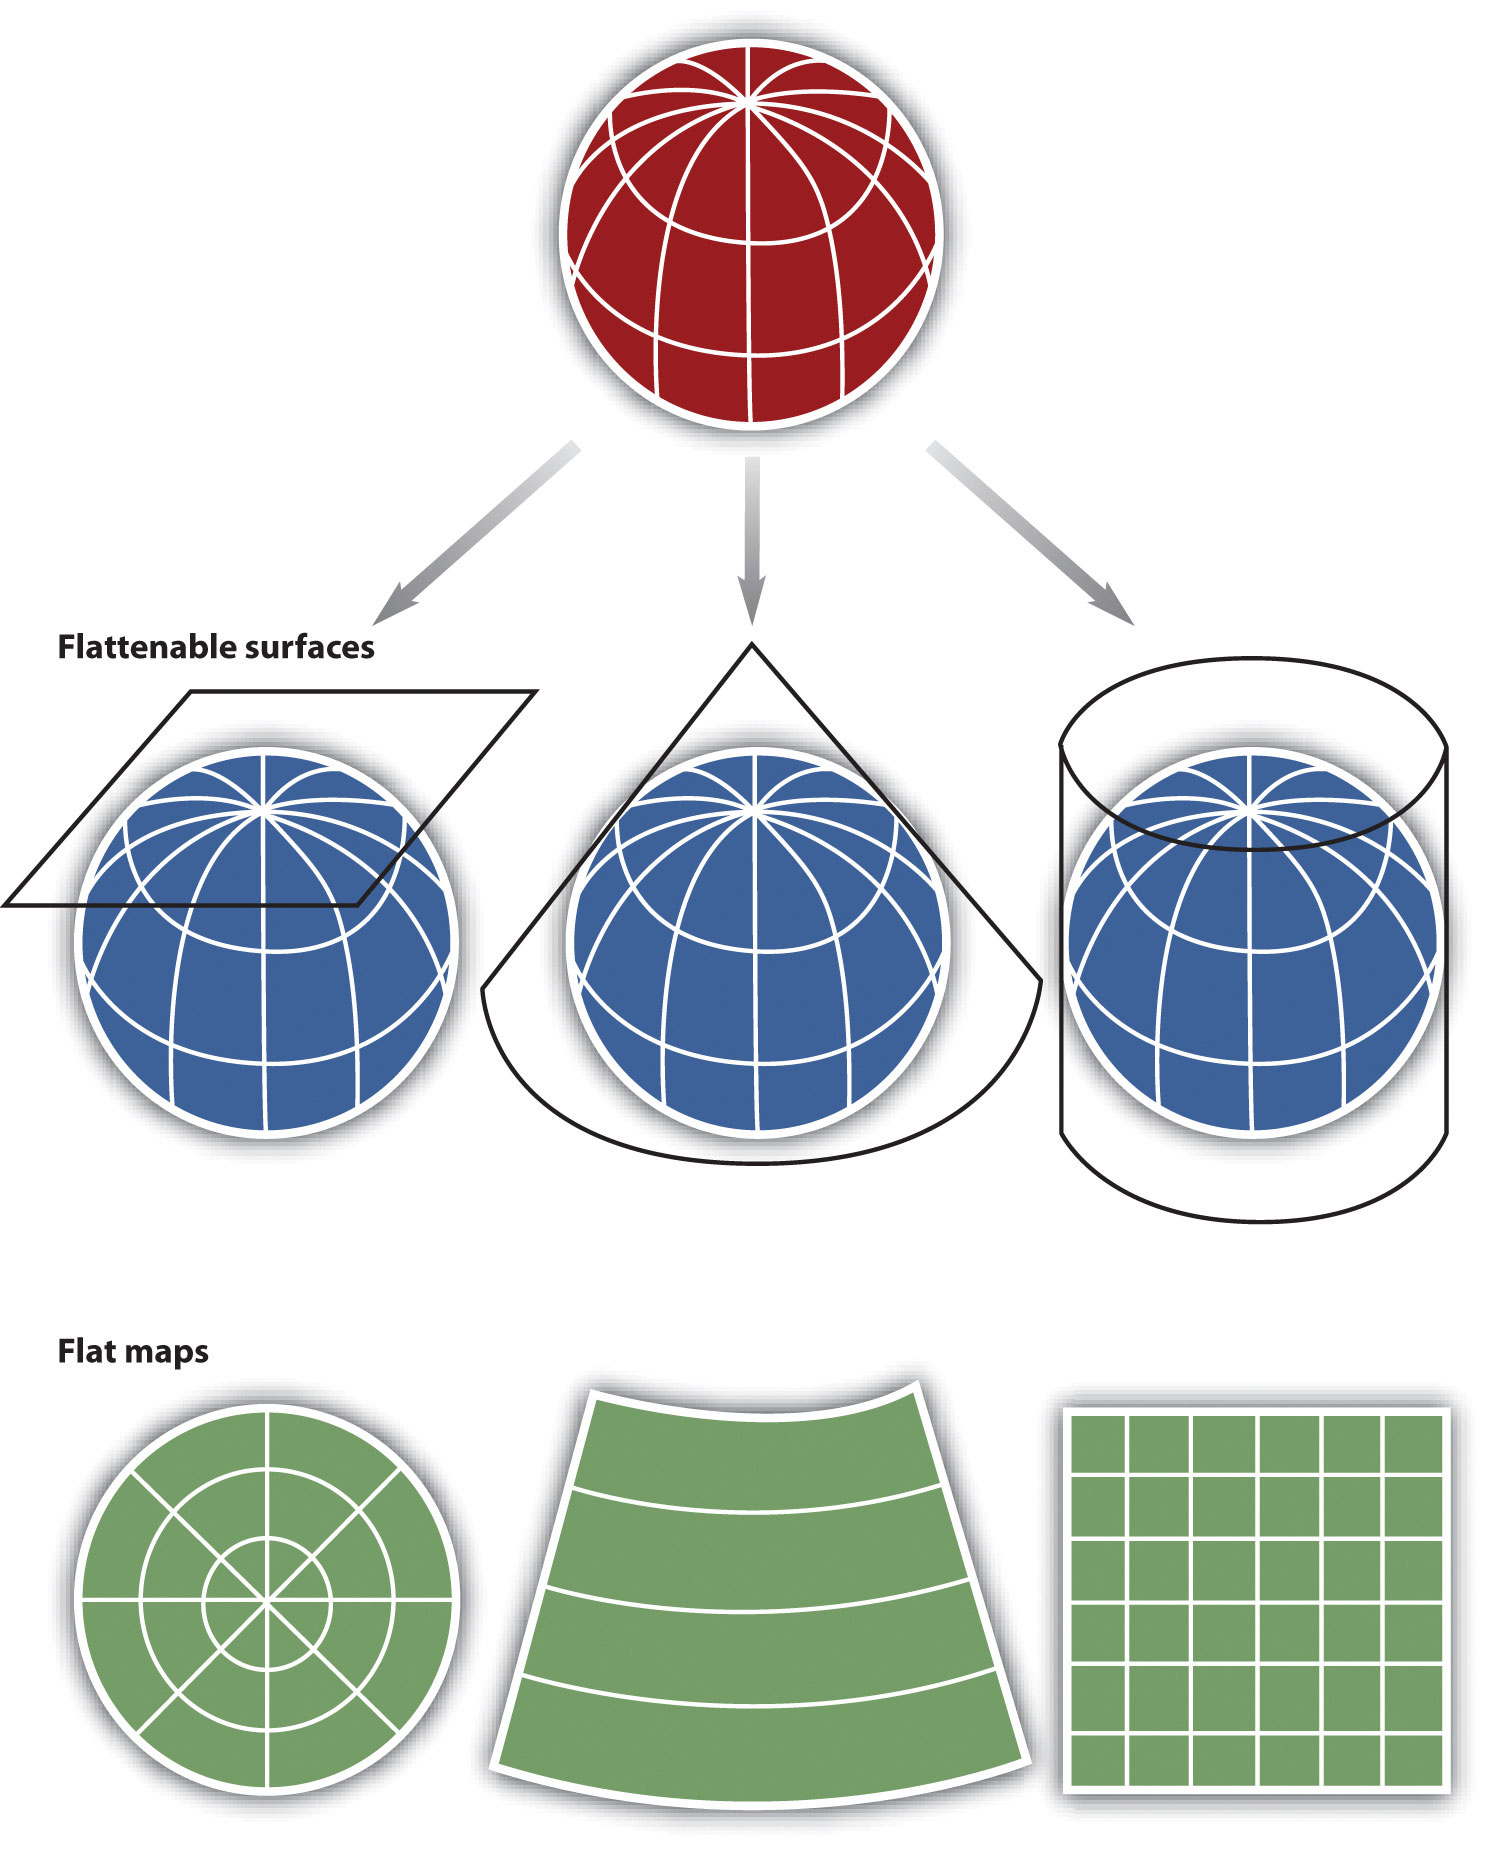
\includegraphics[width=0.65\textwidth]{CRS.png} \\
              \textcolor{gris}{\tiny{Source: \href{https://colorado.pressbooks.pub/makingmaps/chapter/chapter-9-datums-coordinate-systems-and-map-projections/}{Making Effective Maps: Cartographic Visualization for GIS}}} }

              \only<4>{ 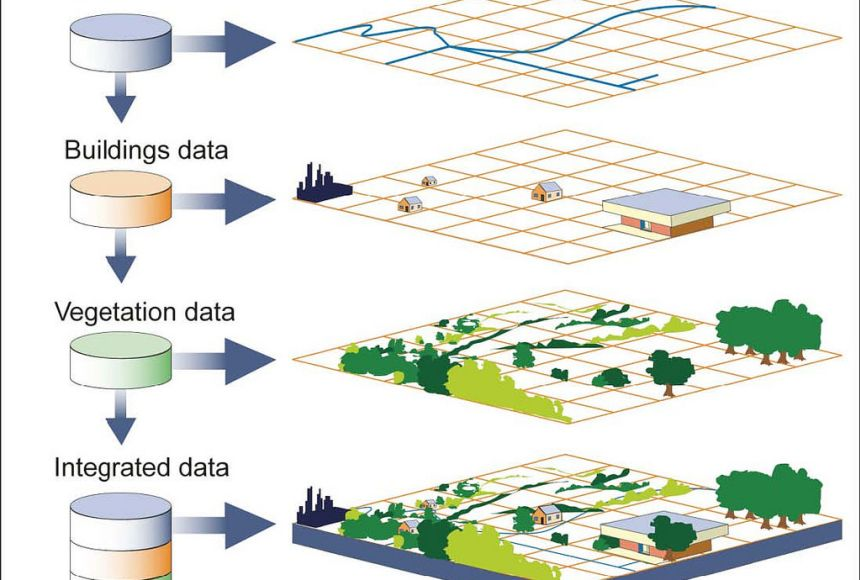
\includegraphics[width=\textwidth]{ gis.jpg} \\
              \textcolor{gris}{\footnotesize{Source: \href{https://education.nationalgeographic.org/resource/geographic-information-system-gis/}{National Geographic}}} }

             \only<5-6>{ \vspace{2.0cm} 
\includegraphics[width=0.2\textwidth]{QGIS.jpg} \\  }
             \only<6>{ \vspace{0.1cm}
\includegraphics[width=0.2\textwidth]{R_logo.svg.png} \\  }
             %\only<5-7>{   \textcolor{gris}{\footnotesize{Source: \href{https://desktop.arcgis.com/en/arcmap/10.3/manage-data/raster-and-images/what-is-raster-data.htm}{Arcgis}}} }
        \end{itemize}
        \end{column}
    \end{columns}
\end{frame}




\begin{frame}
    \frametitle{Tools for Geospatial Analysis}
Using Geospatial data requires high level IT
    \begin{columns}[T]
        \begin{column}{0.5\textwidth}
            \begin{itemize}[<+->]
                \item Data storing and processing architecture: Hadoop, Spark, etc..
                \item Geographic Information System (GIS) software: ArcGIS, QGIS, etc.
                \item Programming languages: R, Python
                \item Web-based mapping platforms: Google Maps API, Leaflet, Mapbox, etc.
            \end{itemize}
        \end{column}
        \begin{column}{0.5\textwidth}
        \vspace{1cm}
            
\includegraphics[width=0.2\textwidth]{R_logo.svg.png}  
\includegraphics[width=0.2\textwidth]{python-logo.png} \\ 
\includegraphics[width=0.2\textwidth]{Tensorflow_logo.svg.png}  
\includegraphics[width=0.2\textwidth]{Pytorch.png}
            
\includegraphics[width=0.2\textwidth]{QGIS.jpg}
        \end{column}
    \end{columns}
\end{frame}

\begin{frame}{Geospatial Data Sources for SDGs}
    \begin{itemize}
        \item \href{https://www.earthobservations.org/sdgs.php}{Group on Earth Observations (GEO)} – Global Earth observation data for SDGs.
        \item \href{https://data.humdata.org/}{Humanitarian Data Exchange (HDX)} – Open geospatial data for crisis and development.
        \item \href{https://www.wri.org/data/wrims-water-data-portal}{World Resources Institute (WRI) – Aqueduct} – Data for water risk and sustainability.
        \item \href{https://datacatalog.worldbank.org/search/dataset/0038272}{World Bank Data – Geospatial SDG Indicators} – Geospatial data for SDG monitoring.
        \item \href{https://www.openstreetmap.org}{OpenStreetMap (OSM)} – Open access geospatial data for global mapping.
        \item \href{https://data.un.org/}{UN Data} – Data platform providing global datasets for tracking SDG progress.
        \item \href{https://land.copernicus.eu/}{Copernicus Land Monitoring Service} – European geospatial data for land and environmental monitoring.
        \item \href{https://sedac.ciesin.columbia.edu/}{NASA SEDAC} – Socioeconomic and environmental geospatial data for sustainable development.
    \end{itemize}
\end{frame}

\section{Conclusion}
\begin{frame}
\frametitle{Conclusion}
    \begin{itemize}[<+->]
        \item Geospatial data analysis is an essential component for understanding spatial patterns and gender-related statistics
        \item[$\hookrightarrow$] See examples soon.
        \item Geospatial information can be linked with traditional data (survey)
         \item[$\hookrightarrow$] Integration and augmentation of data through geospatial reference key
        \item Despite challenges and limitations, advancements in tools and methods enable more effective geospatial analysis.
    \end{itemize}
\end{frame}







\begin{frame} % Cover slide
\frametitle{\textcolor{brique}{[Q\&A]}}
\begin{center}
\Large \textcolor{siap}{ Questions}
\end{center}
\end{frame}


\end{document}


\begin{frame} % Cover slide
\frametitle{ }
\pause
 \begin{itemize}[<+->]
  \item[]
  \item
\end{itemize}
\end{frame}

%%%%%%%%%%%%%%% Last Slide %%%%%%%%%%%%%%%%

\begin{frame}[allowframebreaks]%in case more than 1 slide needed
\frametitle{References}
    {\footnotesize
    %\bibliographystyle{authordate1}
    \bibliographystyle{apalike}
    \bibliography{../../../Visualisation/Visu}
    }
\end{frame}
\end{document}

%\bibliographystyle{authordate1}
%\bibliography{c:/Chris/Visualisation/Visu}
%\end{frame}

\begin{frame}{Title}
\begin{columns}[T]
  \begin{column}{0.7\textwidth}
    \begin{itemize}[<+->]
        \item Sometimes data providers propose a more efficient way to download data
        \item API: "\textbf{A}pplication \textbf{P}rogramming \textbf{I}nterface "
        \item An API is like a waiter in a restaurant
        \item[$\hookrightarrow$ ] He has a menu
        \item[$\hookrightarrow$ ] You can order anything but only on the Menu
        \item[$\hookrightarrow$ ] Data is then served as a structured "ready-to-use" file
     \end{itemize}
     \end{column}

    \begin{column}{0.3\textwidth}
    \begin{center}
      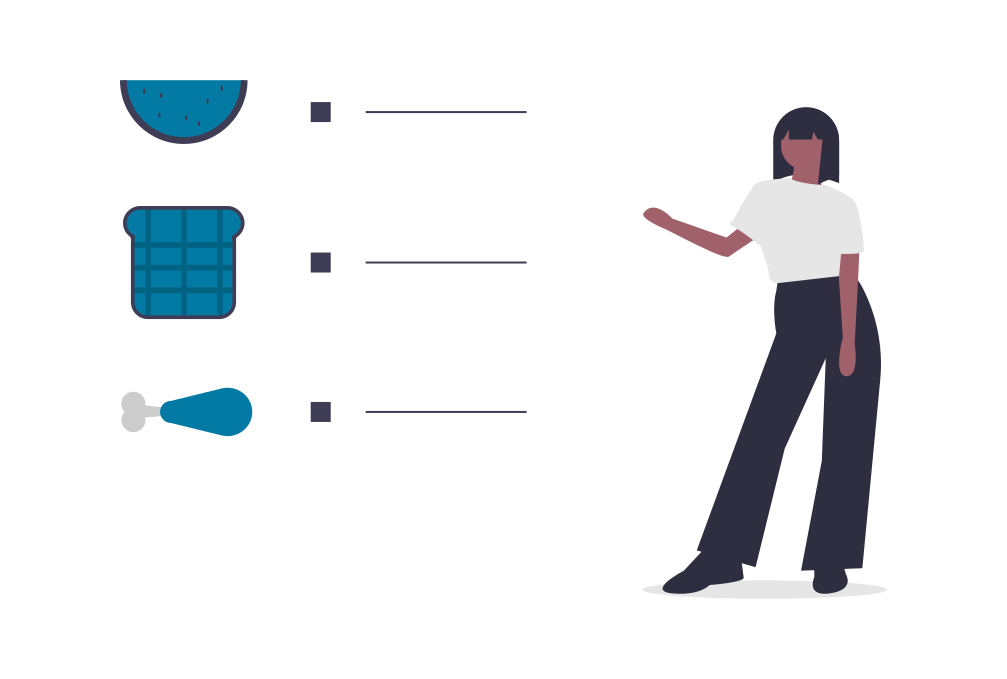
\includegraphics[width=0.9\textwidth]{undraw_diet_ghvw.png}
    \end{center}
    \end{column}
\end{columns}
\end{frame}

